\chapter{Landasan Teori}
\label{chap:definition}

\section{\textsl{Data Mining}}

\subsection{Tahap \textsl{Data Mining}}
Proses pada \textsl{data mining} dapat dibagi menjadi beberapa tahap seperti pada gambar 2.1

\begin{figure}
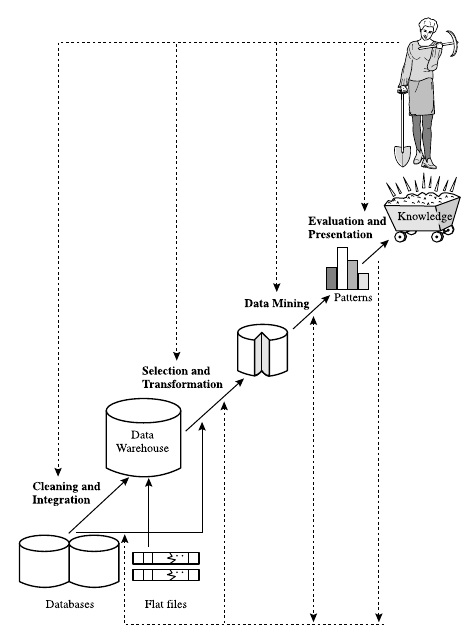
\includegraphics[scale=1]{Gambar/tahapdatamining.jpg}
\caption[Tahap \textsl{Data Mining}, Sumber Data Mining Concepts and Techniques]{Tahap \textsl{Data Mining}, Sumber Data Mining Concepts and Techniques} 
\end{figure}

Terdapat 7 tahap pada \textsl{data Mining}:
\begin{itemize}
	\item \textsl{Data cleaning}
	\item \textsl{Data integration}
	\item \textsl{Data selection}
	\item \textsl{Data transformation}
	\item \textsl{Data mining}
	\item \textsl{Pattern Evaluation}
	\item \textsl{Knowledge presentation}
\end{itemize}

\subsection{\textsl{Data Cleaning}}
\textsl{Data cleaning} merupakan tahap \textsl{data mining} untuk menghilangkan \textsl{missing value} dan \textsl{noisy data}. Pada umumnya, \textsl{data} yang diperoleh dari \textsl{database} terdapat nilai yang tidak sempurna seperti nilai yang hilang, nilai yang tidak \textsl{valid} atau bahkan salah ketik. Nilai-nilai tersebut dapat diatasi dengan cara \textsl{smoothing techniques}. Atribut dari suatu \textsl{database} yang tidak relevan atau redudansi bisa diatasi dengan menghapus atribut tersebut. 

\subsubsection{\textsl{Missing Values}}
\textsl{Missing values} tentu akan mengganggu proses \textsl{data mining} pada komputer dan dapat menghasilkan nilai akhir yang tidak sesuai. Terdapat beberapa teknik untuk mengatasi \textsl{missing values} yaitu
	\begin{itemize}
		\item Membuang tuple yang terdapat nilai yang hilang
		\item Mengisi nilai yang hilang secara manual
		\item Mengisi nilai yang hilang dengan menggunakan nilai konstan yang bersifat umum
		\item Menggunakan nilai rata-rata dari suatu atribut untuk mengisi nilai yang hilang
	\end{itemize}
\subsubsection{\textsl{Noisy Data}}
%\textsl{Noisy data} merupakan nilai yang berasal dari error atau tidak \textsl{valid}. \textsl{Noisy data} dapat dihilangkan dengan menggunakan teknik \textsl{smoothing}. Terdapat 3 metode untuk menghilangkan \textsl{noisy data} yaitu
%	\begin{itemize}
%		\item \textsl{Binning}, merupakan metode pengisian data sesuai dengan proses yang dilakukan pada data tersebut
%		\item \textsl{Regression}, merupakan metode yang mencari persamaan atribut untuk memprediksikan suatu nilai
%		\item	\textsl{Clustering}, merupakan metode pengelompokan dimana ditemukan \textsl{outliers} yang dapat dibuang
%	\end{itemize}

%\subsubsection{\textsl{Data Cleaning as a Process}}
%Tahap pertama pada \textsl{data cleaning} adalah \textsl{discrepancy detection}. Ketidakcocokan dapat dikarenakan oleh beberapa faktor, termasuk desain data yang buruk, kesalahan manusia ketika memasukan data, dan data yang sudah kadarluarsa. Ketidakcocokan ini juga dapat disebabkan tidak konsisten representasi data dan kode atau dikarenakan kesalahan perangkat ketika melakukan pemasukan data.

%Untuk mempermudah pencarian ketidakcocokan tersebut, kita dapat membuat sebuah data yang berisi informasi mengenai data atau biasa disebut \textsl{metadata}. Pada tahap ini, penulisan \textsl{script} bisa ditulis dengan cara masing-masing. Disini, dapat ditemukan \textsl{noise}, \textsl{outliers}, dan nilai-nilai yang tidak cocok atau tidak konsisten.

%Data juga harus diperiksa dengan \textsl{unique rules}, \textsl{consecutive rules}, dan \textsl{null rules}. \textsl{unique rules} mengatakan bahwa setiap nilai dari sebuah atribut harus berbeda dengan nilai yang lain pada atribut tersebut. \textsl{Consecutive rules} mengatakan bahwa tidak boleh ada nilai yang hilang diantara nilai tertinggi dan terendah untuk sebuah atribut, dan semua nilai harus bersifat unik. \textsl{null rules} menspesifikasikan penggunaan nilai \textsl{blanks} atau kosong, tanda tanya, karakter spesial, atau \textsl{string} yang dapat menandakan bahwa nilai tersebut bersifat kosong.

%Tahap deteksi ketidakcocokan ini dapat dibantu juga dengan menggunakan \textbf{data scrubbing tools} dan \textbf{data auditing tools}. \textbf{data scrubbing tools} akan menggunakan sebuah domain data untuk melakukan pencarian ketidakcocokan data dan membetulkan data tersebut dengan menggunakan teknik \textsl{parsing} dan \textsl{fuzzy matching}. \textbf{Data auditing tools} akan mencari ketidakcocokan dengan melakukan analisa data untuk menemukan \textsl{rules}, relasi, dan mendeteksi data yang melanggar hal tersebut.

%Beberapa data dapat diperbaiki dengan cara manual, namun sebagian besar data akan membutuhkan \textsl{data transformation} untuk membetulkan data tersebut.

\subsection{\textsl{Data integration}}
\textsl{Data integration} merupakan tahap menggabungkan data dari berbagai sumber. Sumber tersebut bisa termasuk beberapa \textsl{database}, \textsl{data cubes}, atau bahkan \textsl{flat data}. Tahap ini harus dilakukan secara teliti terutama ketika dalam memasangkan nilai-nilai yang berasal dari sumber yang berbeda. Pada tahap ini, perlu dilakukan identifikasi data apakah data tersebut dapat diturunkan atau tidak agar data yang diperoleh tidak terlalu besar.
\textsl{Data integration} yang baik merupakan integrasi yang dapat memaksimalkan kecepatan dan meningkatkan akurasi dari proses \textsl{data mining}. 

\subsection{\textsl{Data selection}}


\subsection{\textsl{Data Transformation}}
\textsl{Data transformation} merupakan tahap pengubahan data agar siap dilakukan proses \textsl{data mining}. \textsl{Data transformation} bisa melibatkan,
	\begin{itemize}
		\item \textsl{Smoothing}, proses untuk membuang \textsl{noise} seperti yang dilakukan pada tahap \textsl{data cleaning}
		\item \textsl{Aggregation}, proses mengganti nilai-nilai menjadi suatu nilai yang dapat mewakili nilai sebelumnya
		\item \textsl{Generalization}, proses dimana membuat suatu nilai yang bersifat khusus menjadi nilai yang bersifat umum
		\item \textsl{Normalization}, proses dimana suatu nilai dapat diubah skalanya menjadi nilai yang lebih kecil dan spesifik
		\item \textsl{Attribute construction}, proses membuat atribut baru yang berasal dari beberapa atribut untuk membantu proses data mining
	\end{itemize}
--tanyakan!!!-->Proses \textsl{smoothing} merupakan proses yang sama seperti pada tahap \textsl{data cleaning}.<---tanyakan!!!--

\subsubsection{\textsl{Data Reduction}}
Proses \textsl{aggregation} dan \textsl{generalization} akan dilakukan dalam bentuk proses \textsl{data reduction} dan \textsl{Data Cube Aggregation}.
\textsl{Data reduction} dan dilakukan untuk mendapatkan nilai yang representif namun tetap menjaga keakuratan hasil \textsl{data mining}. Terdapat beberapa cara dalam mengimplementasikan \textsl{data reduction} yaitu
	\begin{itemize}
		\item \textsl{Data cube aggregation}
		\item \textsl{Data subset selection}
		\item \textsl{Dimensionality reduction}
		\item \textsl{Numerosity reduction}
		\item \textsl{Discretization and concept hierarchy generation}
	\end{itemize}

\subsubsection{\textsl{Data Cube Aggregation}}
\textsl{Data cube} menyimpan semua informasi agregat dalam bentuk kubus, guna melakukan analisis. gambar 2.1 merupakan contoh dari \textsl{data cube}. Setiap sel, terdapat nilai data agregat yang saling berhubungan untuk menjadi data multidimensional point. \textsl{Data cube} dapat membuat proses \textsl{data mining} menjadi cepat untuk diakses dan membuat kesimpulan data. 

\subsubsection {\textsl{Attribute Subset Selection}}
\textsl{Attribute subset selection} merupakan salah satu cara melakukan \textsl{data reduction} dengan menghilangkan atribut-atribut yang tidak relevan atau data yang redudansi. Hal ini dapat mempermudah pencarian pola dikarenakan banyak atribut yang muncul akan berkurangnya. 

\subsubsection {\textsl{Dimensionality Reduction}}
\textsl{Dimensionality Reduction} merupakan metode pengurangan nilai secara random dengan cara melakukan konversi data. Jika data original dapat dibuat ulang dari data yang sudah dikompresi tanpa kehilangan informasi, maka akan dikatakan \textsl{lossless}, namun jika hanya mendapatkan data pendekatannya saja, akan disebut lossly [1].

\subsubsection {\textsl{Numerosity Reduction}}
\textsl{Numerosity Reduction} merupakan metode dimana data diganti atau ditentukan dengan cara parametik atau nonparametrik.

\subsubsection {\textsl{Discretization and Concept Hierarchy Generation}}
lewat dulu

\subsection{\textsl{Data Mining}}
\subsection{\textsl{Pattern Evaluation}}
\subsection{\textsl{Knowledge Presentation}}

\section{\textsl{Spatial and Spatiotemporal}}